\documentclass[12pt,letterpaper,english,bibliography=totocnumbered,abstract=on]{scrartcl}

\usepackage{indentfirst}
\usepackage{appendix}
\usepackage{fullpage}
%\usepackage{subfiles}
\usepackage[T1]{fontenc}
\usepackage[latin9]{inputenc}
\usepackage{color}
\usepackage{babel}
\usepackage{verbatim}
\usepackage[unicode=true,pdfusetitle,
bookmarks=true,bookmarksnumbered=false,bookmarksopen=false,
pdfborder={0 0 0},pdfborderstyle={},backref=false,colorlinks=true]
{hyperref}
\hypersetup{linkcolor=blue,citecolor=blue,urlcolor=blue}

\usepackage{booktabs}
\usepackage{multirow}
\usepackage{adjustbox}
\usepackage{threeparttable}
\usepackage[table]{xcolor}
\usepackage{csquotes}
\usepackage{soul} % for hiliting text: \hl
% old style is authoryear
\usepackage[backend=biber, style=numeric, maxbibnames=99]{biblatex}
\addbibresource{mylibrary.bib}
\addbibresource{CRB.bib}

\usepackage[disable]{todonotes}

\usepackage{graphicx}

% Prevent page breaks within paragraphs
% https://tex.stackexchange.com/questions/21983/how-to-avoid-page-breaks-inside-paragraphs
\widowpenalties 1 10000


\begin{document}
\titlehead{US Forest Service Forest Health Protection Grant Progess Report 4}
\title{Improving Coconut Rhinoceros Beetle Breeding Site Detection Using Harmonic Radar}
\author{Aubrey Moore, University of Guam}
%\date{Submitted December 30, 2020\\Revised January 28, 2021}
\maketitle
\begin{description}	
	\item[GRANTEE:] Aubrey Moore, University of Guam 
	\item[GRANT YEAR:] 2020
	\item[GRANT NUMBER:] 20-DG-11052021-227
	\item[GRANT PROGRAM:] Forest Health Protection
	\item[GRANT EXPIRATION DATE:] 2022-12-31 (extended)
	\item[DATES COVERED BY THIS REPORT:] 2022-01-01 through 2022-06-30
	\item[GRANT STATUS:] Active
\end{description}	

\textbf{Note to Reader:} Significant changes from the previous report are indicated by \textbf{bold-faced text}.

\bigskip

\begin{footnotesize}
\url{https://github.com/aubreymoore/Harmonic-Radar/raw/master/FS-CRB-HR-report4.pdf}
\end{footnotesize}


\newpage{}
\tableofcontents{}

\newpage

\begin{figure}
	\centering
	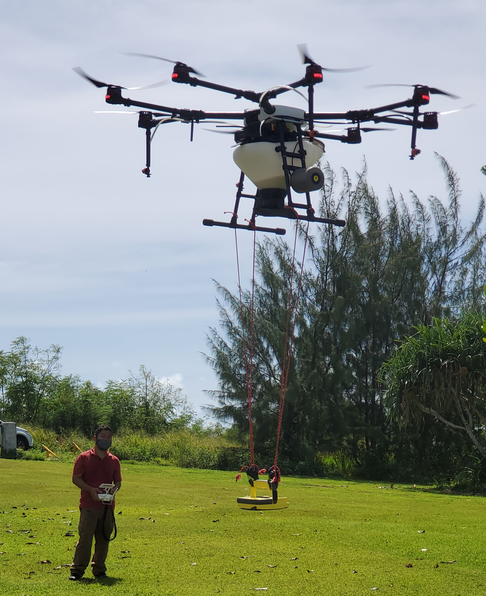
\includegraphics[width=0.7\linewidth]{drone}
	\caption{RECCO harmonic radar device suspended from an agricultural drone piloted by Dr. Glenn Dulla, Guam Department of Agriculture.}
	\label{fig:drone}
\end{figure}

\clearpage


\section{OBJECTIVES AND SPECIFIC ACTIVITIES} 

%List the objectives individually that were included in the grant narrative.  Under those objectives include specific activities that occurred during the report timeframes.   

The objective of this grant project is to evaluate harmonic radar as an alternative to radio tracking for CRB breeding site detection. Detection of CRB breeding sites is essential for CRB control and eradication.

Previously, we successfully tracked CRB to cryptic breeding sites using miniature radio transmitters. However, the high cost of radio tags (>\$100 each) and short shelf life and field life of nonreplacable batteries (about 1 month and one week, respectively) make this technique too expensive for routine surveys to detect CRB breeding sites. 

A promising alternative technology is harmonic radar. Harmonic radar tags do not require a battery. They are inexpensive (about \$1 each) and they have unlimited shelf-life and field life. We are evaluating hand-held harmonic radar equipment and tags manufactured by RECCO in Sweden. Rescuers use the hand-held units to rapidly locate victims wearing tags sown into their clothing. RECCO technology has been used to track other insects but has not yet been tried with CRB.

Our objective is not to track CRB tagged beetles in real-time, but to discover the end points of tags several days or even weeks after release of tagged beetles. We anticipate that tags will accumulate at breeding sites.

Here is the plan from the approved grant proposal:

\medskip
\colorbox[gray]{0.9}{\parbox{\textwidth}{
	\textbf{Schedule of Activities (2020)}
	\begin{description}
		\item[March-April:] Tag fabrication and testing at EMU.
		\item[April-early May:] Capture, flight test, and mark CRB at UoG.
		\item[May:] Conduct field releases and tracking of tagged CRB (two week intensive fieldwork period).
		\item[June-August:] Data analysis.
		\item[August-December:] Manuscript(s) and final report preparation.  Discuss findings with state agencies.  Make presentations at scientific meetings.  Plan further research with cooperators to implement findings in monitoring and control efforts.
	\end{description}
}}
\medskip

Progress to date includes:
\begin{itemize}
\item Procurement of harmonic radar equipment and tags
\item Tag fabrication (soldering antennae to diodes) in Matt Siderhurst's lab.
\item Preliminary field testing of equipment on Guam.
\item \textbf{Published our research idea as a preprint in the Research Ideas and Outcomes Journal (\href{https://doi.org/10.3897/rio.8.e86422}{Moore and Siderhurst 2022}). This article will be peer reviewed.}
\item \textbf{Continued to investigate the idea of mounting our harmonic radar transceiver on an aerial drone to facilitate automated surveys over large areas (See Methods Development section below). }
\end{itemize}

The most important activity in our work plan is to conduct field releases and tracking of tagged CRB over a two week intensive fieldwork period. This intensive fieldwork will be performed on Guam in collaboration with Matt Siderhurst's team of students who have experience in tracking insects with harmonic radar. (We are following an approach similar to what we did in the radio-tracking feasibility study \href{https://academic.oup.com/ee/article/46/1/92/2633399?login=false}{Moore et al. 2017}). This fieldwork activity has not yet been scheduled because of COVID-19 travel restrictions (See section \ref{impediments} for details.). Otherwise we are prepared to proceed. \textbf{Our field trial is now planned for July 2022.}

\subsection{Methods Development}

The RECCO hand-held harmonic radar device we are using is designed for ground-based location of tags. We are collaborating with Dr. Glenn Dulla, Guam Department of Agriculture, to test the idea of mounting the device on a drone to allow efficient downward-looking scans over large areas. The idea is to mount the RECCO device on a drone which is programmed to fly a defined search path. A digital recorder cabled to the RECCO's headphone jack records the audio signal from the device and the drone's GPS  records location. Georeferencing is done by matching timestamps in the audio recording with timestamps in the GPS data. Postprocessing generates a map of signal strength with peaks indicating probable tag locations requiring confirmation by ground searches.

Preliminary tests are promising:
\begin{itemize}
	\item Used digital recordings of the RECCO's audio output to locate tags (See Technical Report: \href{https://github.com/aubreymoore/Harmonic-Radar/raw/master/experiments/techreport/techreport.pdf}{Using a Cell Phone as a Datalogger for Handheld Harmonic Radar})	
	\item Flown the RECCO harmonic radar device attached to a drone (Fig. \ref{fig:drone})
	\item Based on initial flight tests we determined that the audio data recorder we were using was too heavy for use on the drone. We purchased a much smaller and light audio data recorder. Walk tests with this recorder show that we can locate harmonic radar tags by correlating audio recordings with GPS data (Fig. \ref{fig:211109003}).
	\item \textbf{On June 9, 2022 we flew a drone with our harmonic radar transceiver suspended beneath it. Audio output from the transceiver was recorded on a small audio data recorder. By correlating audio data with the drone's GPS log, we were able to locate harmonic detector tags on the ground (See \href{https://github.com/aubreymoore/Harmonic-Radar/raw/master/experiments/2022-06-09-drone/techreport.pdf}{technical report}).}
\end{itemize}

\begin{figure}[h]
	\centering
	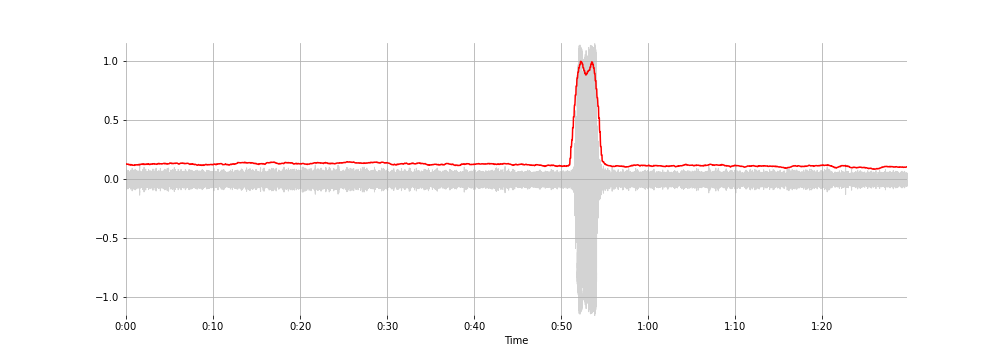
\includegraphics[width=\linewidth]{211109_003.png}
	\caption{Audio output from a RECCO harmonic radar device recorded using a Zoom F2 field recorder. This was a walk test along a linear transect in which a harmonic radar tag had been placed. Location of the tag in the recording is clear.}
	\label{fig:211109003}
\end{figure}

\clearpage

\section{OUTPUTS} 

%Each Output listed in your grant narrative addressed individually.
%
%1) Output 1: list the output and what was accomplished.
%2) Output 2: list the output and what was accomplished.
%3) Etc.
%
%If output includes positions funded: (who, how long, type of work)
%
%If output includes Acres treated, include target species, number of acres and location 
%
%If output includes Acres surveyed, include target species, number of acres and location 
%
%Description and dollar value of equipment purchased, 
%
%Number of personnel trained. 

On December 18, Aubrey Moore made a presentation on the technology used in this project at a meeting of the Guam Beekeepers Association (GBA). Members of the GBA and the Guam Department of Agriculture are interested in using harmonic radar to track greater banded hornets (GBH), \textit{Vespa tropica}, to their nests so that they can be destroyed. GBH, a recently arrived invasive species which raids honeybee hives, is a serious threat to Guam's nascent beekeeping industry.

\section{MONITORING \& EVALUATION}

%If post-treatment monitoring has been completed, provide the results, especially results that show effectiveness of treatments.  
%
%List any project evaluations that took place to determine whether goals and Statewide Strategies are being met.

Nothing to report.

\section{BUDGET EXPENDITURES}

%Include budget table showing the expenditures (Personnel/salary costs, supplies purchased, contracts, etc.) that occurred during the reporting period

\begin{tabular}{lrrl}
	\hline
	Category & Budget & Spent & Note \\
	\hline 
	Equipment and supplies & \$8,000 & \$316.93 & Miniturized audio field recorder and hardware \\ 
	Travel & \$12,000 & \$0 \\ 
	Admin. fee & \$3,000 & \$0 \\ 
	\hline 
\end{tabular} 

\section{PROBLEMS ENCOUNTERED DURING THIS REPORTING PERIOD}
\label{impediments}

%Explain delays, adverse conditions or changed costs that significantly impair the ability to meet grant objectives.  If necessary, prepare a separate formal request for an extension of the grant period:

Progress on this project was impeded by COVID-19 travel restrictions which prevented collaborators from visiting Guam to participate in field work. Further delayed by delay was caused by Government of Guam \textit{stay at home} orders. 

The University of Guam was officially closed from March 20 to May 10 2020 and again from August 16 2020 to January 15 2021.

\textbf{COVID travel restrictions during the current reporting period did not allow Dr. Siderhurst and students to visit Guam to perform the planned field work on schedule. Guam still has extremely high local transmission of COVID due to delayed arrival of the OMICRON variant. However, quarantine for fully vaccinated visitors from the mainland is no longer required. Travel arrangements have been made for Dr. Siderhurst and students experienced with using harmonic radar to track insects to visit Guam during July 2022 to complete planned field trial.}  

\section{CHANGES PLANNED}

% (If the scope of the objectives would change, or if more that 10\% of the total grant budget would change object class categories, prepare a separate formal request to amend the grant):

Nothing to report.

\section{CIVIL RIGHTS}

% - any activity that demonstrates Title VI compliance with civil rights requirements, such as documentation of outreach to underserved groups, public education documents in languages other than English, etc

Nothing to report.

\section{ATTACHMENTS}

% (photos of activities are very helpful, also electronic copies of survey and treatment maps, copies of developed brochures or posters, etc.):

None.

\section{PLANS}

% for work to be performed during next reporting period:

Nothing to report.

\end{document}
